\documentclass[twoside,openright]{report}

\usepackage[english]{babel}
\usepackage[a4paper]{geometry}
\usepackage[sc]{mathpazo}
\usepackage[utf8]{inputenc}
\usepackage[T1]{fontenc}
\usepackage{Alegreya}
\usepackage{microtype}
\usepackage{lipsum}
\usepackage{graphicx}
\usepackage{titling}
\usepackage{imakeidx}
\usepackage{parskip}
\usepackage{cite}
\usepackage{url}
\usepackage{fancyhdr}
\usepackage{appendix}
\usepackage{fancyref}
\usepackage[nottoc]{tocbibind}
\usepackage[hidelinks]{hyperref}
\usepackage[toc,section=chapter]{glossaries}

\makeindex
\makeglossaries

\pagestyle{fancy}
\renewcommand{\headrulewidth}{0pt}

\newglossaryentry{banana}{
	name=banana,
	description={A tropical, edible, yellow fruit with a mushy interior}
}

\newglossaryentry{press}{
	name=press,
	description={A gesture where a single finger touches the screen}
}

\newglossaryentry{tap}{
	name=tap,
	description={A gesture where a finger touches the screen for a short while, then immediately lifts up}
}

\newglossaryentry{press and hold}{
	name={press and hold},
	description={A gesture where the screen is pressed and the finger is held in place for a certain time}
}

\newglossaryentry{swipe}{
	name={swipe},
	description={A gesture where the finger is moved while pressing the screen}
}

\newglossaryentry{canvas}{
	name={canvas},
	description={The plane on which all the visual components are placed (not just the visible part)}
}

\newglossaryentry{visible part}{
	name={visibile part},
	description={The part of the map currently visible within the screen edges}
}

\newglossaryentry{function block}{
	name={function block},
	description={A visual block representing a haskell function}
}

\newglossaryentry{GHC}{
	name={Glasgow Haskell Compiler},
	description={A popular and actively-developed Haskell compiler toolchain, and base of the official Haskell Platform, see \url{http://haskell.org/ghc}}
}

\newglossaryentry{REPL}{
	name={read-eval-print-loop},
	description={An interactive (usually command-line) interface that allows executing programming language expressions without having to do an intermediate compilation step}
}

\newglossaryentry{FXML}{
	name={FXML},
	description= {An XML-based language that provides the structure for building a user interface separate from the application logic of your code}
}

\newglossaryentry{TactileAPI}{
	name={TactileAPI},
	description= {An API written for JavaFX that enables easy multi-touch supports for dragging and dropping elements in a Pane}
}


\title{Report}
\author{
     Martijn Bruning
\and Kristel Hartsuiker
\and Jan-Jelle Kester
\and Wander Nauta
\and Derk Snijders
}
\date{\today}

\begin{document}

\newcommand{\code}[1]{\texttt{#1}}

\renewcommand*\rmdefault{ppl}
\renewcommand*\sfdefault{ppl}
\urlstyle{same}

\begin{titlepage}
    {\Huge \thetitle} \\
    \vfill
    \begin{center}
        \makebox[\textwidth]{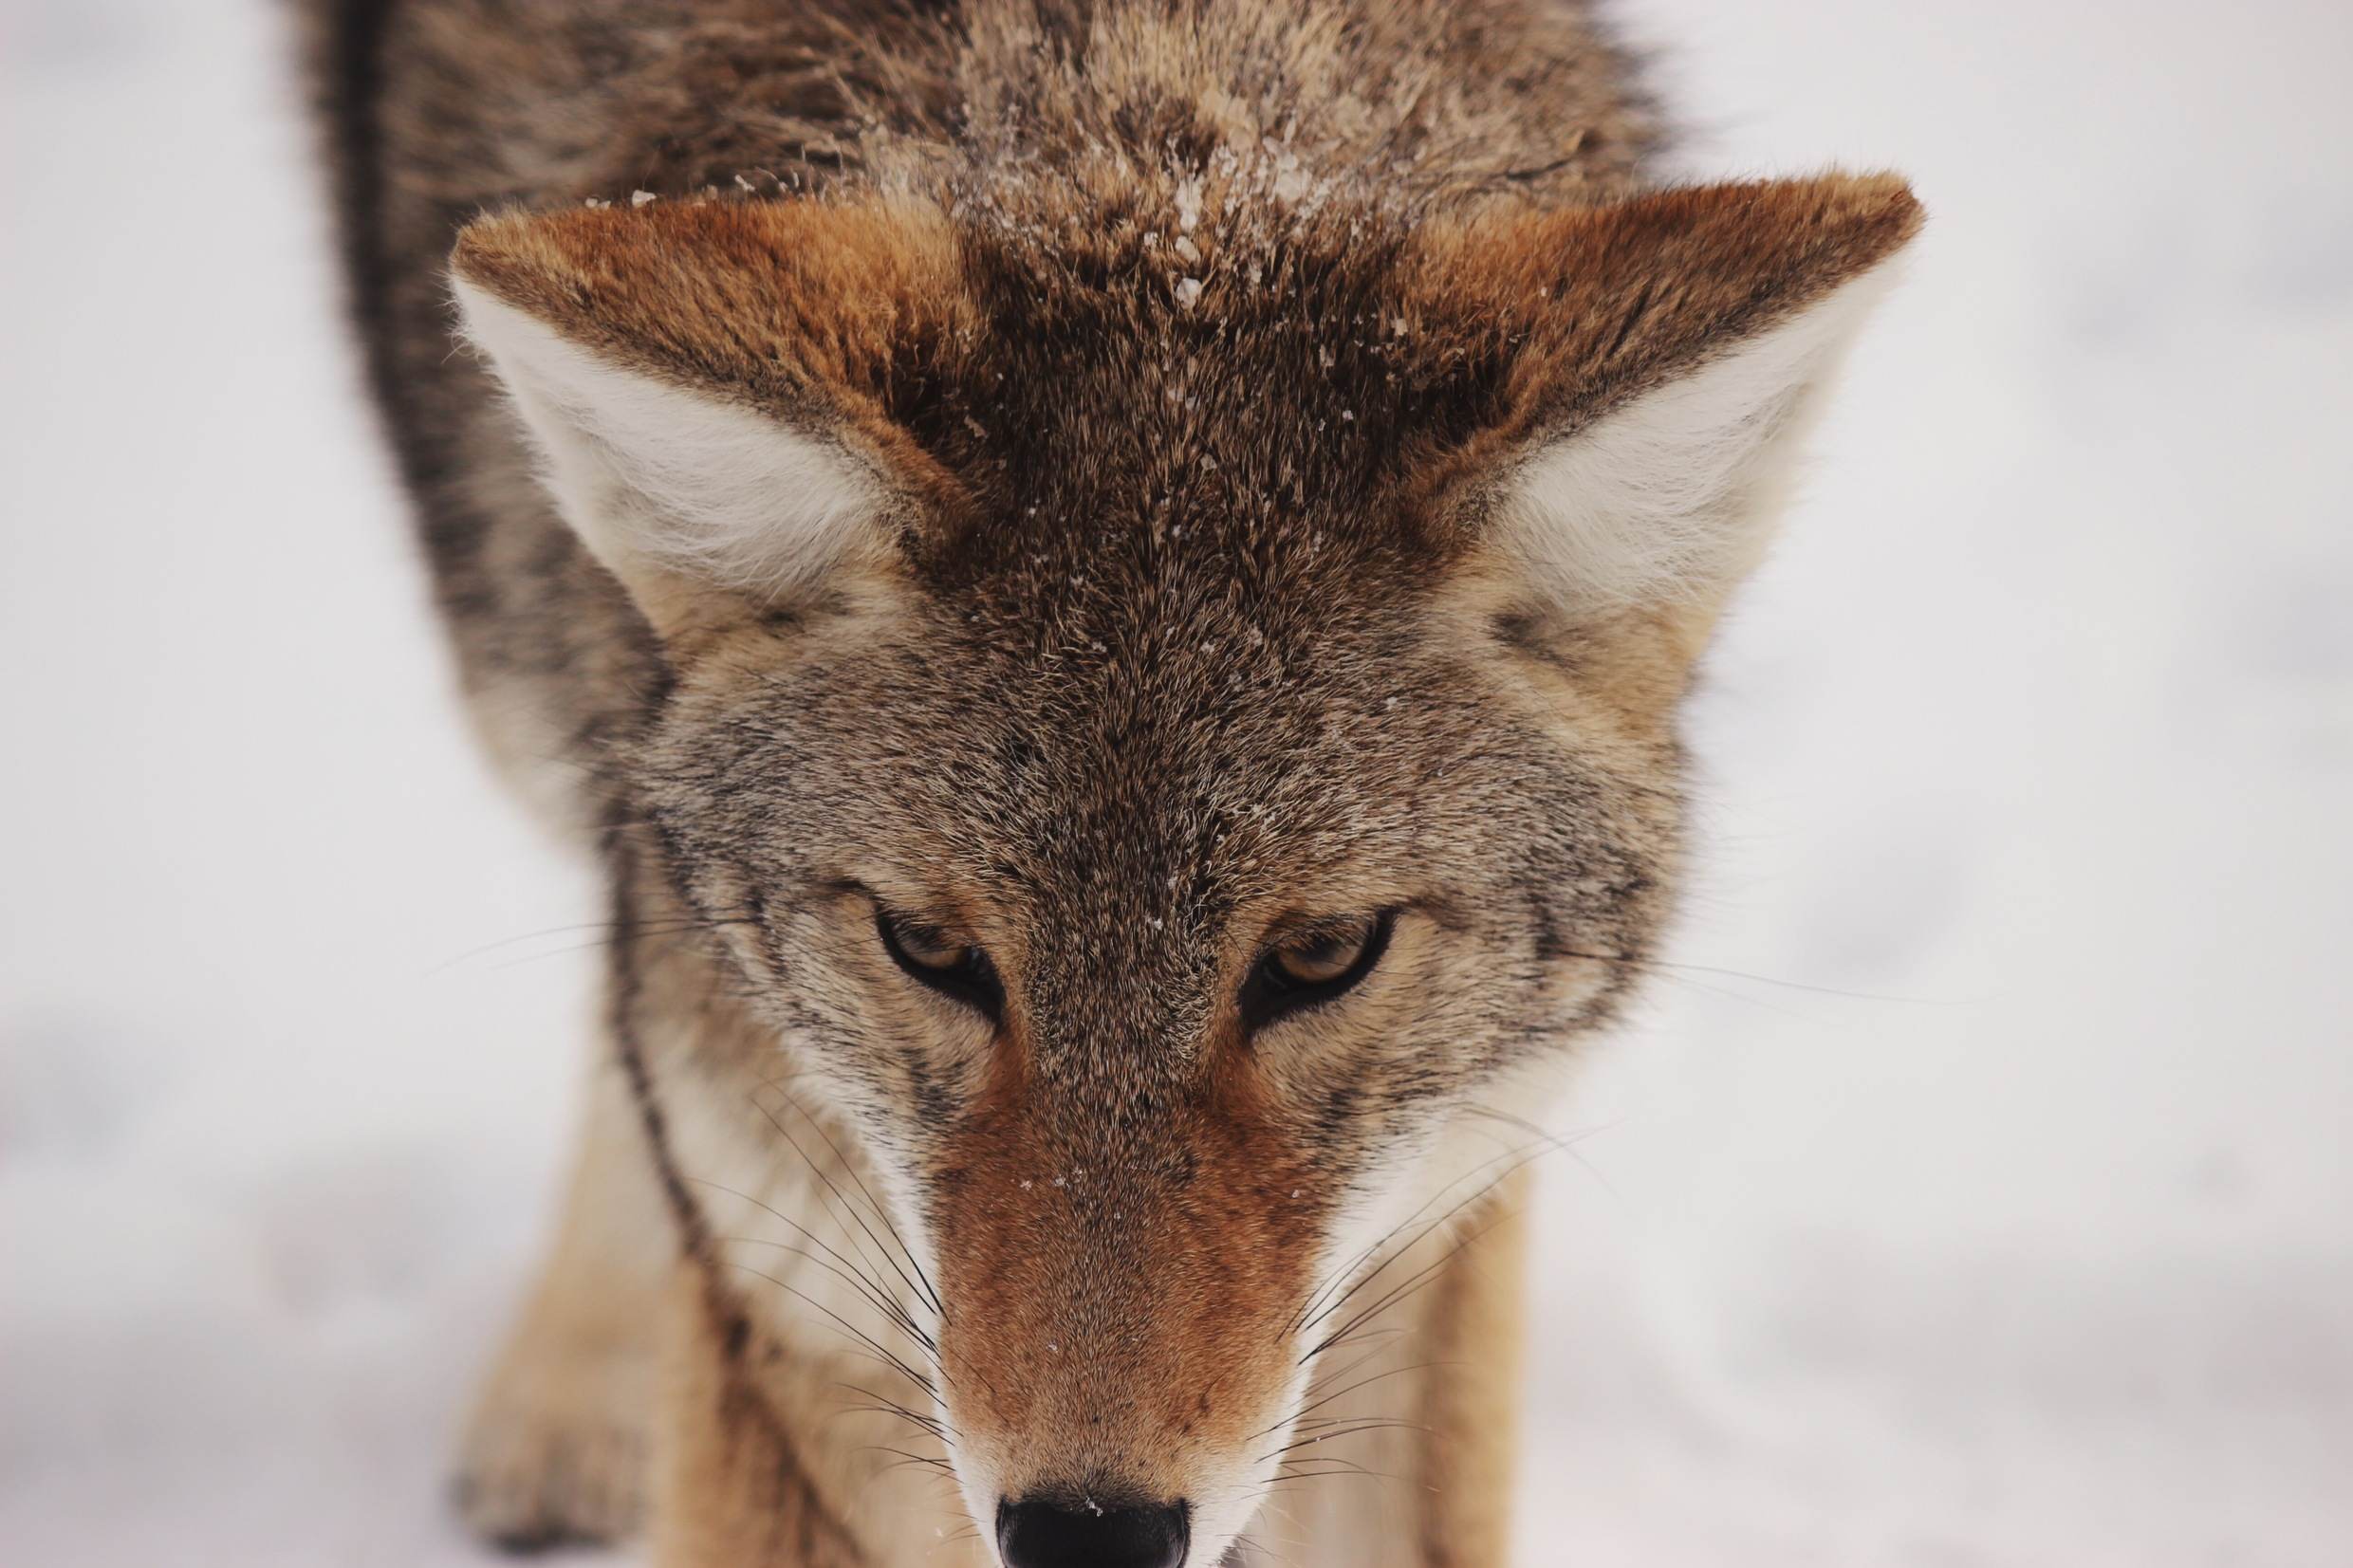
\includegraphics[width=230mm]{Images/front}}
    \end{center}
    \vfill
    {Design project}\\
    \theauthor \\
    \thedate
\end{titlepage}

% Inhoudsopgave
\tableofcontents

\chapter{Summary}


\chapter{Introduction}

Programming has always been an activity which is done on a computer with a keyboard. Despite the existence of different visual programming languages, like Blender, there are no programs in which well known programming languages like Java, Haskell or C(++) can be visually implemented. 

In this project we have (attempted) to make an application in which the programming language Haskell can be visually implemented.
%aanvullen als het project af is

In this report the different aspects of the developing process are being discussed. The upcoming chapters discuss the requirements analysis, the design process, the implementation process (front end \& back end), how the application has been tested, the evaluation of the process and the conclusions. 

\chapter{Process and tools}

In the early stage of the project, we settled on the process and tools we were going to use during the project. An evaluation of the process we used, with details on what worked out well for us and what didn't, can be found in \fref{chap:Evaluation}. \index{process}

\section{Buzzword-compatible process}

It was quickly decided that the development process we were going to use for the project should be entirely buzzword-compatible: no outdated waterfall models, no long and tedious iterations, but a quick, nimble development process. \index{buzzwords}

\subsection{Sprints}

Development goals were to be decided on for short periods of time. We dubbed these periods sprints, in line with Agile terminology. Every sprint was to be two weeks long. (During the project, we had some one-week sprints, for example when we expected that there would be more time available than in usual weeks.) \index{sprints}

\section{Tasks and responsibilities}

\subsection{Process tasks}

In the very first meeting, we divided process-related tasks and responsibilities. Derk was to be the chairman, leading the biweekly meetings; Jan-Jelle became the chief of communications, responsible for keeping the customer and mentor happy and up to speed; Martijn was assigned to guard the project's progress; Wander was volunteered to do code integration and keep an eye on code quality, and Kristel offered to keep the records and write minutes during meetings. \index{tasks}

Every process task was assigned to two team members, with one member carrying the responsibility and one member acting as a back-up in case the primary member wasn't available for whatever reason.

\subsection{Implementation and design tasks}

For the very first part of the project, Martijn, Kristel and Derk were assigned to start working on the program's front end design. Wander and Jan-Jelle were to tackle the beginnings of a usable back end, that is, getting the program designed in the front end to run. This split kept existing during most of the project because of the familiarity with the code.

\section{Code tools}

Software projects have a tendency to become quite large, and Java projects more than most. We decided to use some tools to help us manage the code base.

\subsection{Maven}

Larger Java projects usually have dependencies. These dependencies can also have dependencies. To make sure every team member was using the same versions of the libraries the project, we decided to use Maven, a Java build tool. Using Maven as a standardized build process also allowed team members to work from their preferred environment: the back end crew preferred IntelliJ IDEA by JetBrains, while the front end developers worked mostly in Eclipse. \index{Maven}

\subsection{Git, GitHub and GitHub Flow}

For the version control system, we decided on git, with the central repository stored on GitHub. \index{git} \index{GitHub}

As for a branching model, we decided on GitHub Flow\cite{githubflow}. In this model, small, independent changes are published to their own branches, tested, checked, then proposed as a Pull Request. At this point the person responsible for code integration (either Wander or Jan-Jelle) reviewed the code and merged it into the master branch. \index{GitHub Flow} Additionally, GitHub was used as issue tracker.

\subsection{Travis}

It is no use having automated unit tests if they are never executed. To make sure we would get alerted to broken tests quickly, we decided to use Travis CI with the project to build every (pushed) change and run the unit tests. Travis automatically sends email notifications when a build fails. It also integrates with GitHub's pull request feature, showing the build status there as well to help keep broken code out of the master branch. Travis has proven to be a very useful tool. \index{Travis} \index{continuous integration}

\section{Process tools}

We also used quite a few tools to help us manage the project itself.

\subsection{Trello}

The layout of a Trello project with horizontally placed containers which hold vertically aligned cards makes it a good tool for maintaining sprints. Trello also supports check-off lists, assigning people to cards and a built-in calendar with iCal export so important events can show up in everyones agenda. \index{Trello}

\subsection{Google Drive}

Meeting minutes, design descriptions and related documents were stored in Google Drive to make sure every team member had easy access to them, when needed. \index{Google Drive}

\subsection{Google Groups}

We decided to set up a mailing list using Google Groups to make it easier to share important messages and files. Google Groups has an additional benefit that it allows one to browse and search old messages, making it something of a paper trail. \index {Google Groups}


\chapter{Requirements Analysis}

The first step in creating an application or program was defining the requirements. In order to do this, we planned meetings with our client. Against our expectations the client did not have many demands to the project. He wanted us to be free in the design and implementation. The main goal of the project was not creating a program, which is 100\% finished and could be used right away, but to explore the possibilities of the client's ideas (a proof of concept).

To start however, we needed something more than just an idea. We needed a base from which we could work. This resulted in a set of requirements, which we defined based on the ideas of our client.

\section{Target audience}

How to divide the requirements in necessary and desirable requirements depends on the kind of target audience for which the application is designed. \index{audience} \index{target audience}

In this project the focus lies mainly on users who already know how to program in Haskell. This includes people who are just starting with Haskell.
The program should aid these users in creating an overview of their program and informing them about (possible) mistakes without the user having to write a complete program and then compile it.

Furthermore, the users are generally advanced computer users and therefore do not require an in-depth explanation on how to operate a program. The users will also have a basic understanding of touch gestures, most likely obtained through the use of a smart phone or tablet.

\section{Hardware}

The program will be designed to use on a large multi-touch screen with a screen resolution of 1920x1080 pixels, but should also work with a smaller (for example laptop) screen and a mouse. The program should be efficient enough to run on average modern-day hardware. The client provided a desktop computer and multi-touch screen for reference.

\section{Requirements}

For this project, the requirements can be divided in three subgroups, namely: visual requirements, functional requirements and multi-touch requirements. In the following subsections each of the groups will be discussed. In some cases a requirement fits in multiple groups; in these cases the best fitting group has been chosen to contain this requirement.

\begin{enumerate}
\item \subsection*{Visual requirements}

\begin{enumerate}
	\item The structure of the visual program must logically represent the structure of a regular Haskell program.
		\begin{enumerate}
			\item Haskell functions are represented by a separate element.
			\item The program has to be able to show a compact notation for a program using stacked and nested blocks.
			\item Blocks must be movable to prevent them from overlap.
		\end{enumerate}
	\item The program must allow functions/blocks to be interconnected.
		\begin{enumerate}
			\item Function arguments must be connected individually.
			\item A block has a single output which can be the final result of the function or the result of a partial application.
		\end{enumerate}
	\item The user interface design must be minimalistic.
	\item The user interface must be resizeable.
	\item Actions performed by the user must give feedback.
	\item Errors and warnings (for example type errors) must be easily recognizable.
	\item In case blocks and lines overlap, lines must be drawn behind the blocks.
	\item Users must be able to select functions to using a touch screen only.
\end{enumerate}

\item \subsection*{Functional requirements}

\begin{enumerate}
	\item The program has to support incomplete programs.
	\begin{enumerate}
		\item It must be possible to have blocks or groups of blocks that are not interconnected.
		\item The program must give feedback (for example type errors) about incomplete programs.
	\end{enumerate}
	\item It must be possible to define custom Haskell functions. This includes a free choice in number of arguments, type and name of the function.
	\item The program must generate executable Haskell code from the visual representation. This implies that objects in the visual representation have a precise meaning.
	\item The program must perform real-time type checking of the connected functions.
	\item The program must be able to show the real-time output at any point in the program. The user may be required to perform a small number of actions to achieve this.
	\item The program must be expandable by different developers.
	\begin{enumerate}
		\item The source code must be documented properly.
		\item The design choices must be documented properly.
	\end{enumerate}
\end{enumerate}

\item \subsection*{Multi-touch requirements}

\begin{enumerate}
	\item Users with large fingers should be able to use the program. This may be achieved with either large visual elements or touch areas larger than the visual element.
	\item Actions may use gestures that are simple and have a short learning curve.
	\item It should be possible to use the program with more than one person at the same time on the same touch screen.
	\item It should be possible to use the program with only one hand.
	\item The program should only require a keyboard as input method when absolutely necessary.
\end{enumerate}

\end{enumerate}

\chapter{Design}

This chapter contains a high level description of the design choices made in the process of creating Viskell.
The specific implementation details are discussed in chapter \ref{chap:implementation} on page \pageref{chap:implementation}.

\section{User interface}

The entire user interface consists of components floating around on a drag and drop canvas, the \code{CustomUIPane}. Menus can be opened on empty \gls{canvas} and from their different blocks can be created and interacted with.

\subsection{Graphical design}

\subsubsection{Blocks and lines}
Among the other components floating around in the canvas, blocks and the way they are connected make up the Haskell program. We chose blocks since this is a logical element for users, they can be seen as small calculators that perform a specific action.

Blocks have input and output anchors that can be used to create connections from one block to another, essentially representing the Haskell program flow. Input anchors are positioned on the top of a block, the output anchor on the bottom side. The inside of a block is defined by the block itself, for functions this is a name and the types of the arguments it expects.

We chose to make a distinction between three kinds of blocks, each having their own colour to make them easily recognizable.
The first kind is an output block, which represents a constant value. \index{value block} \index{output block}
This input block can be connected to other blocks which can use its outputted value as input.
Besides the most basic output block, the value block which takes a string as input for creation and then automatically detects the type, there is also a slider available. \index{slider block}

The second kind of block displays the program's output (yet is called an input block, since it receives input).  \index{input block}
There are multiple versions, ranging from a simple block that displays the string representation of its input to a graph block which can show a function. \index{graph block}

The third kind of block is a function block. This block has a number of inputs, a single output, and a knot defining the number of inputs that need to be connected. \index{function block}

The number of inputs can be changed by moving the knot left or right, over the function's arguments.
This allows for passing (partially applied) functions as input for other functions. \index{partial application}
A useful example for this is the \code{map} function.

During the project, many different ideas where pitched for blocks, eventually we went with something a bit different from the client's initial idea. Some more information about this can be found in \ref{chap:Evaluation}.

\begin{figure}[p]
	\centering
	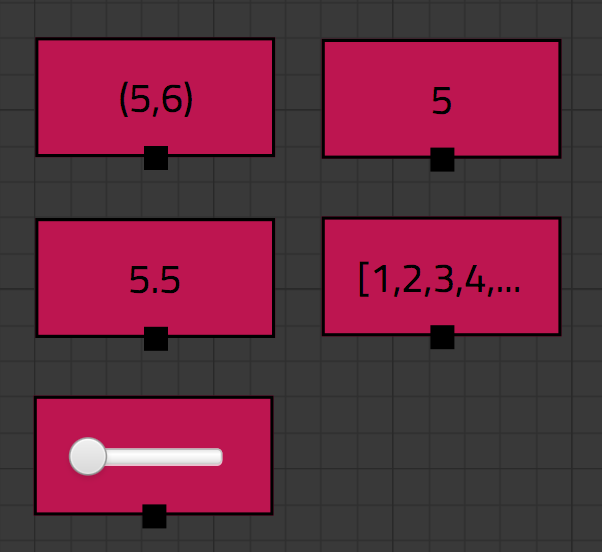
\includegraphics[scale=0.5]{Images/blocks-inputs}
	\label{fig:blocks-inputs}
	\caption{Different input blocks}
\end{figure}

\begin{figure}[p]
	\centering
	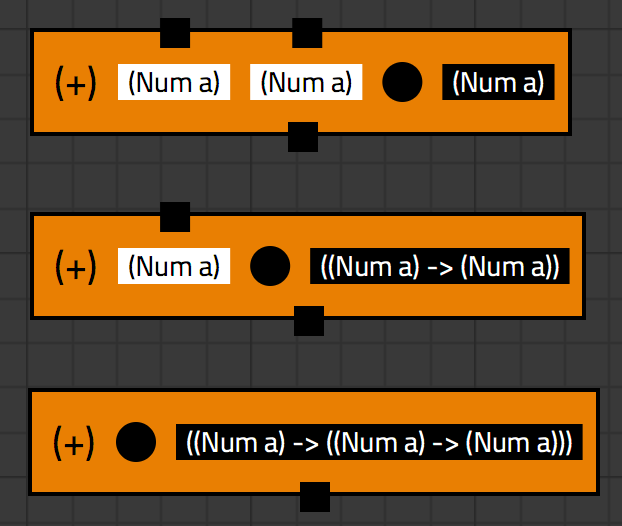
\includegraphics[scale=0.5]{Images/blocks-bowties}
	\label{fig:blocks-bowties}
	\caption{Partial application of functions}
\end{figure}

\begin{figure}[p]
	\centering
	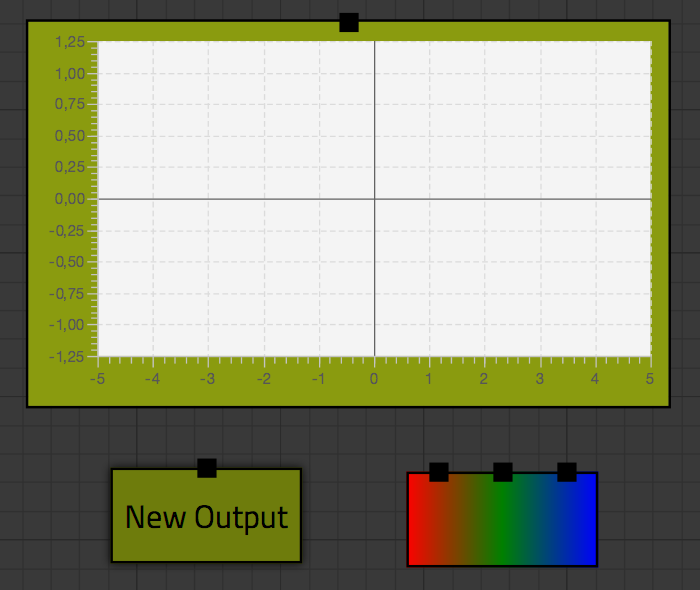
\includegraphics[scale=0.5]{Images/blocks-outputs}
	\label{fig:blocks-outputs}
	\caption{Different output blocks}
\end{figure}

\begin{figure}[p]
	\centering
	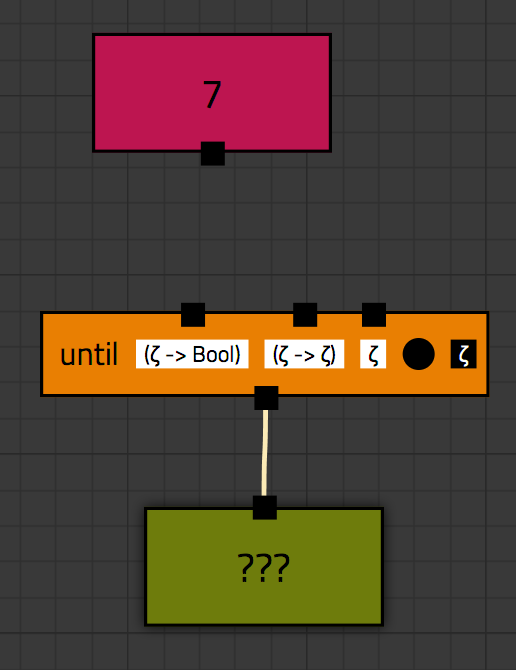
\includegraphics[scale=0.5]{Images/blocks-example}
	\label{fig:blocks-example}
	\caption{Different kinds of blocks}
\end{figure}

%TODO position these images better

\subsubsection{Errors}

An important part of Viskell is representing programming errors.
Instead of requiring users to stop editing and compile a complete program, Viskell re-compiles whenever a change in the program is made. Due to this, type errors can be displayed as soon as a user connects two blocks. These errors are represented as a coloured, red, line and coloured, red, type in the target block's input arguments. An icon is displayed inside the incorrectly connected anchor as well to help colour blind users.

\subsubsection{Menus}

During the design process many ideas for the menus came up.
One of the first ideas was to have a circular menu. \label{circular_menu} \index{circle menu}
The advantages of the circular menu would be that the orientation of the device would not have any influence on the usability of the menu.
This would makes using the program on a large multi-touch table with multiple users easier.
However, the implementation of the menu would take too much time and on top of that the client preferred something more like his initial sketches. The idea of a circular menu was therefore dropped.

\begin{figure}[p]
	\centering
	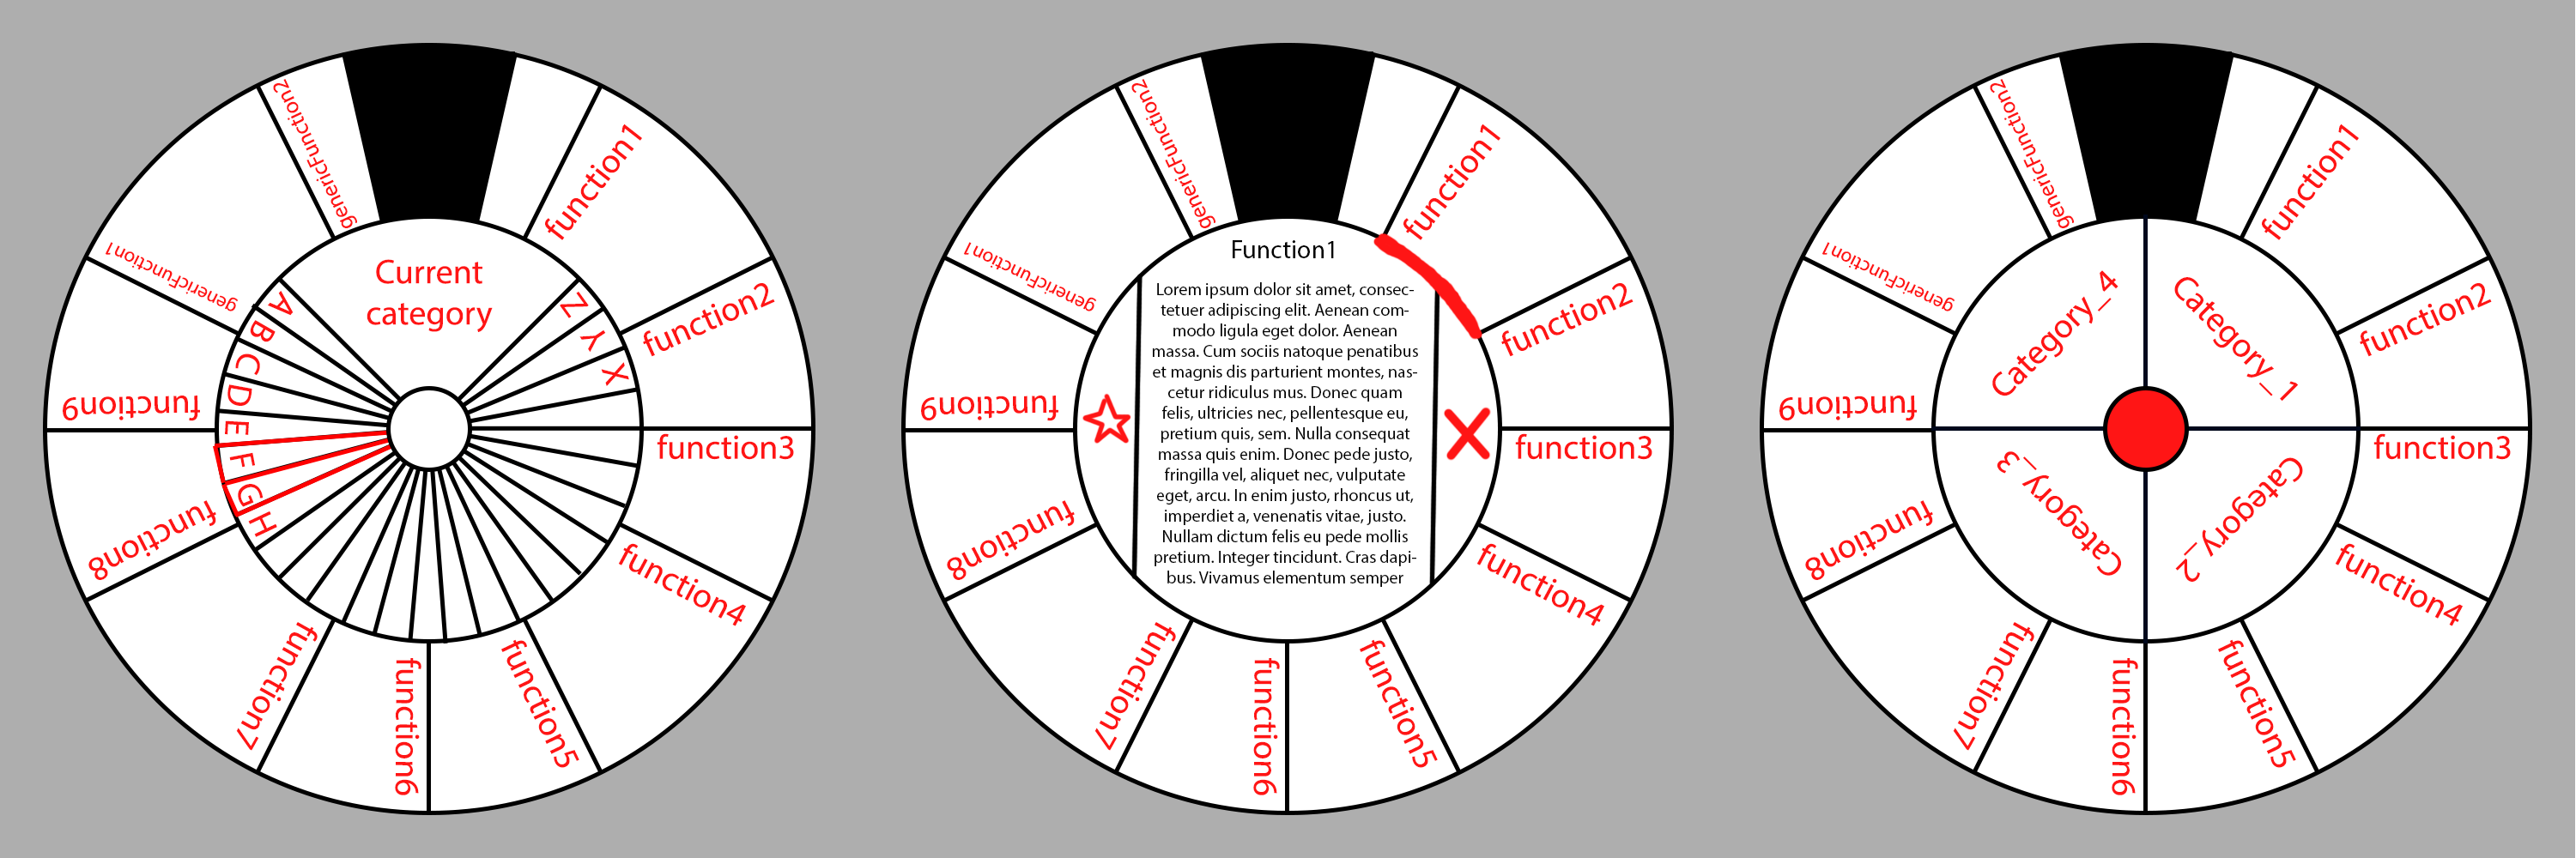
\includegraphics[width=\textwidth]{Images/circlary}
	\label{fig:circlary}
	\caption{Concept of circular menu}
\end{figure}
\begin{figure}[p]
	\centering
	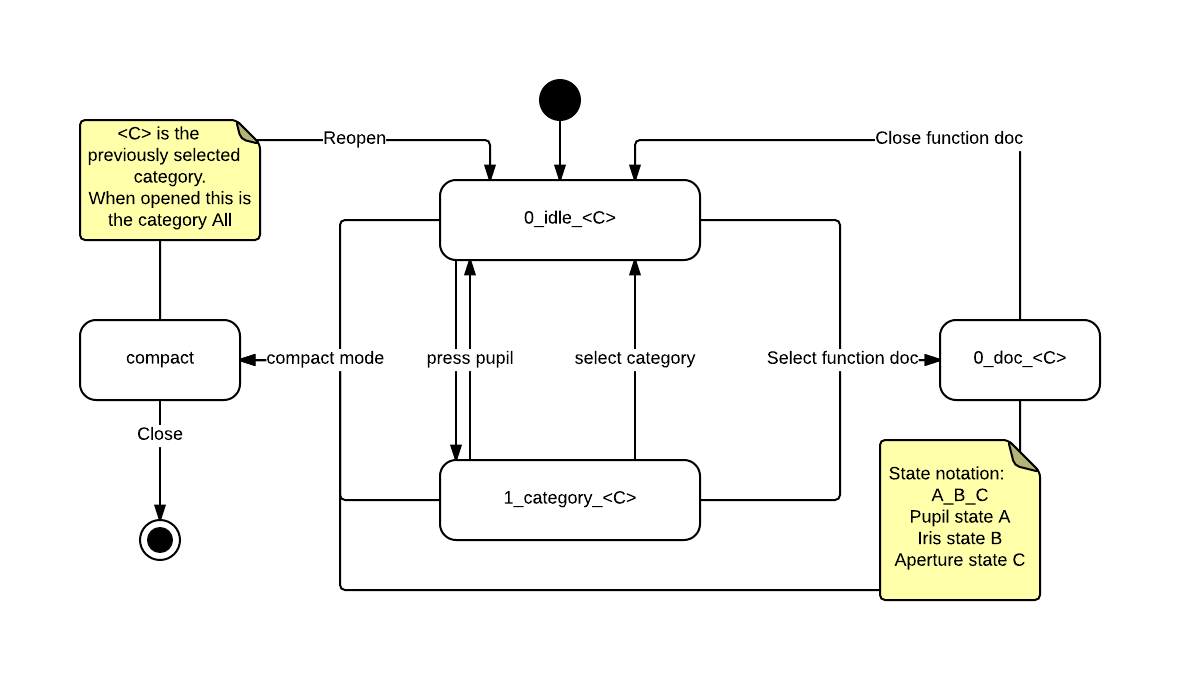
\includegraphics[scale=0.5]{Images/diagram-circlary}
	\label{fig:diagram-circlary}
	\caption{Circular menu diagram}
\end{figure}

The final menu design has two separate menus, one for adding new blocks and one for contextual options on existing blocks.

The primary menu (or `function menu') uses `drawers' for the categories of the functions. \index{primary menu} \index{function menu}
This way it is easy to find functions even without an extensive knowledge of Haskell.
In- and output blocks and the function definition block can be created using buttons at the bottom of the menu.
This location is chosen to make them quickly available.
The primary menu can be opened multiple times at once and moved around the screen so multiple users can work on a single program. An additional benefit of having a floating menu is that screen size never impacts reachability of the menu, as opposed to having a menu stuck to one of the sides.

\begin{figure}[p]
	\centering
	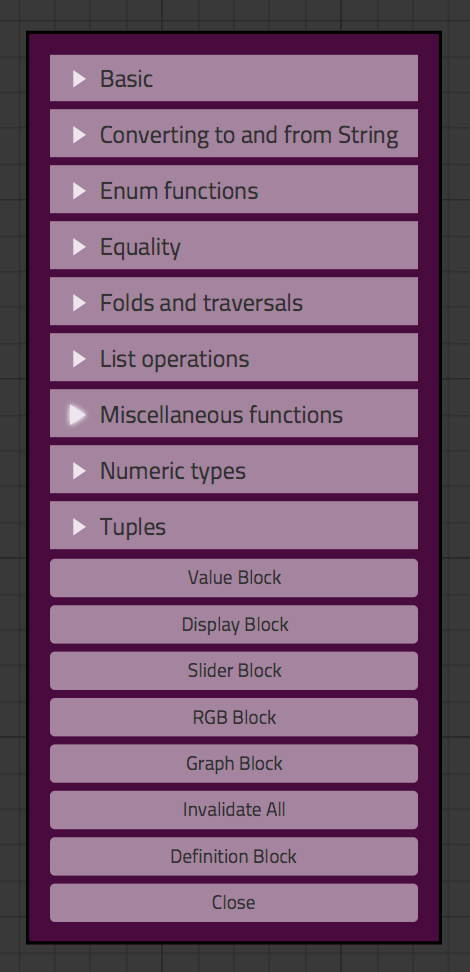
\includegraphics[scale=0.5]{Images/menu}
	\label{fig:ui-menu}
	\caption{Primary menu}
\end{figure}

The context menu is compact so is does not take up too much space. \index{context menu}
It contains clear icons which represent different actions for the single selected block, like delete.
The icons are large enough to touch, even for people with large fingers.

\begin{figure}[p]
	\centering
	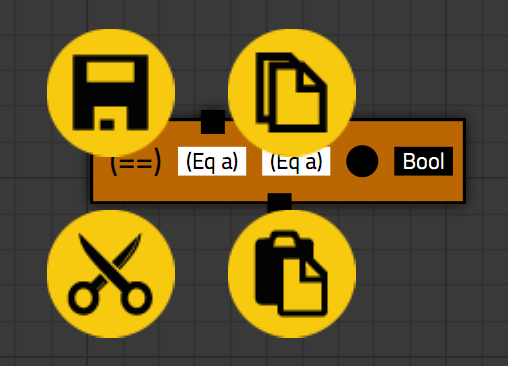
\includegraphics[scale=0.5]{Images/blocks-menu}
	\label{fig:blocks-menu}
	\caption{Context menu}
\end{figure}

\subsubsection{Colour scheme}

The background colour of the canvas is a type of dark grey.
This is chosen because it is less tiring for the eyes than white and allows for a high contrast.
The background also incorporates a grid pattern so users can align elements on the screen if they like to.

All other components feature a cheerful colour scheme.
This colour scheme provides good contrast with the background and solid recognizability for the different kinds of blocks.

\subsection{Behaviour and interaction design}

Our goal was to provide an easy to use and intuitive (multi) touch interface, with a very easy learning curve. To achieve this we looked at the way smart phones provided touch interaction and tried to stick to their philosophy on the matter.

A very clear rule in that philosophy is to always have to perform as little actions as possible to do what you want to do, we strived to achieve this with Viskell. An example of this is the ability to edit a connection. Instead of having to delete one first and then create a new one, we added the ability to edit a connection, combining what would otherwise be 2 actions into a single action. Our menus were also constructed with the same goal in mind.

To make sure that the user has a good overview of what he is doing we focussed on as much and as direct live feedback as possible. This can be seen in the way a type mismatch is displayed. The idea was to also be able to quickly undo incorrect actions, by using an undo button, which should also keep the learning curve low.

An activity diagram of the interaction a user can have with Viskell is shown in Figure \ref{fig:activitydiagram} on page \pageref{fig:activitydiagram}. As can be seen in the figure, the number of actions a user can perform is not very large (amount of blocks in the 'User' column). This confirms the short learning curve we wanted to achieve. Although the number of actions is not very large, the number of possibilities in the program at a given point is quite extensive. This is visualised by the many lines in the activity diagram. This means that you can almost do anything from any state in the program.

The fact that it is almost possible to do anything from anywhere is probably a (positive) side effect of our goals regarding multi touch. While the client's wants on the matter were a bit vague, we eventually settled on the requirement that all single user actions needed to be able to be concurrently performed in the case of multiple users. This resulted in almost all actions being able to happen concurrently. Despite our attempts, some actions still do not support multi touch (for example opening a function menu), yet this should be relatively easy to solve in the future.

\begin{figure}[p]
	\centering
	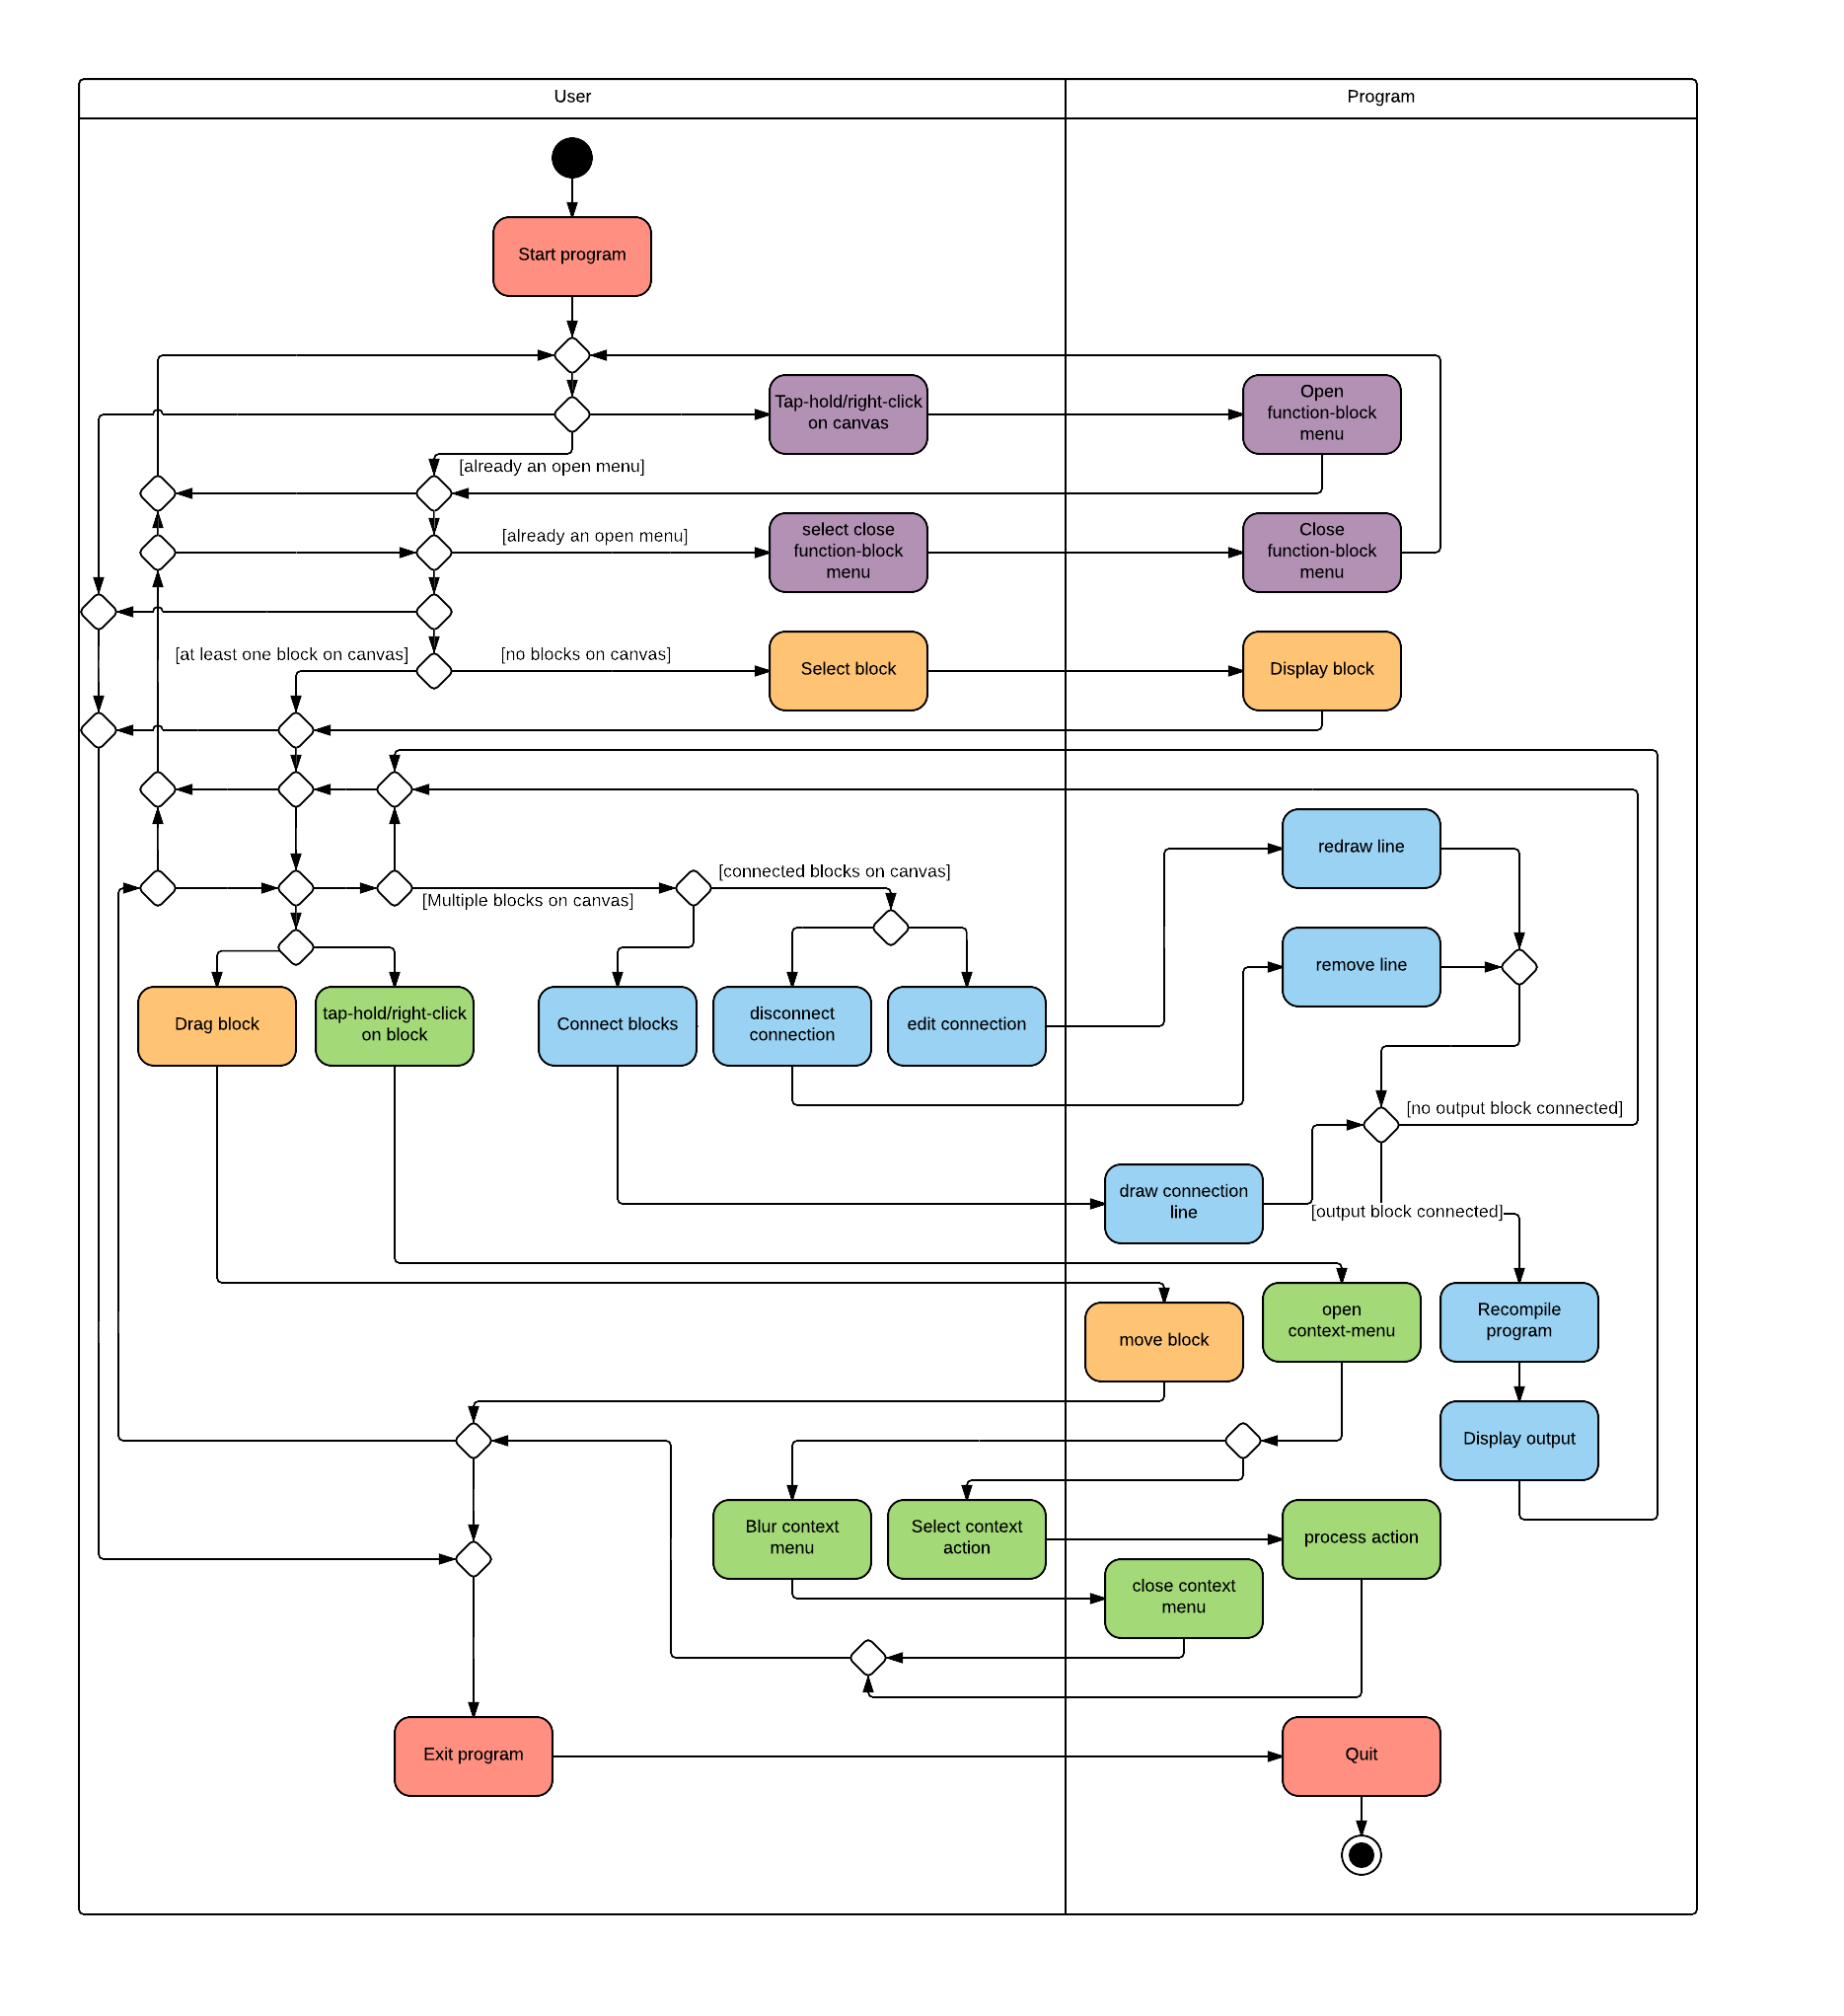
\includegraphics[width=\textwidth]{Images/activitydiagram}
	\label{fig:activitydiagram}
	\caption{Activity diagram}
\end{figure}

\section{Languages and libraries}
Viskell is written in Java 8, which comes bundled with JavaFX. \index{JavaFX}
Java 8 is chosen because it, unlike Java 7, still receives public updates at the moment of writing and allows us to make use of some of the new features in this version.

Viskell uses TactileFX, a JavaFX touch screen library developed at the University of Twente.
The client wanted the program to use this library, which also means that Viskell had to use Java and JavaFX.

Furthermore, the following libraries have been used:

\begin{itemize}
	\item Antlr 4 (\url{http://www.antlr.org/})
	\item Guava (\url{https://github.com/google/guava})
	\item JFXtras (\url{http://jfxtras.org/})
\end{itemize}

\section{High-level architecture}
Viskell consists of two parts, a front end and a back end. \index{front end} \index{back end}
The front end is responsible for providing a user interface, handling user input, displaying error messages, and communicating with the back end.
The back end consists of a representation for Haskell code in Java, an interface to GHCi (see \ref{GHCi} on page \pageref{GHCi}) and functionality to make working with the back end easier.
This separation is made to make development and debugging for the part that generates Haskell code easier.
It also makes using the user interface for a different purpose a bit easier, although the user interface has been designed specifically for our use case.

\section{Front end architecture}
We designed Viskell with multi-touch interfaces in mind. \code{\gls{TactileAPI}}, a public library, was made available to us to assist with multi-touch interfacing. Since TactileAPI is based on javaFX, Viskell is also based on javaFX. \code{CustomUIPane}, our extension of \code{TactilePane}, has many of the same responsibilities of a main \code{Window} and stores most of the program state.
Listeners are attached to \code{CustomUIPane} to monitor \code{Mouse-} and \code{TouchEvents} that are directly responsible for the interaction with Menus.

While the general listeners are controlled from the \code{CustomUIPane}, components often have specific listeners attached to them.
This is done so that the gestures could easily change the state of the component it belonged to. Wherever possible, complex handlers were given their own class such as \code{AnchorHandler}. Since the project is aimed at providing support for multi-touch we needed additional functionality to accommodate this. A solution that is often chosen is the mapping of an input identifier to performed actions.

Placed on \code{CustomUIPane} are components, detailed further on. For all of the Components we made use of the FXML language available in javaFX.

\subsection{Gestures}
Interaction with the user interface is possible through touch gestures on the touch screen or by using a mouse. Since JavaFX only supports three different multi-touch events: pressed, moved and released, we had no choice but to base as much as possible of the interaction on these 3 events. Equivalent mouse events are used to preserve symmetry and ease of development. Some more advanced mouse gestures are used (for example when opening menus), these can be accessed with touch from synthesized touch events. These more advanced gestures do not however work correctly with multi-touch.
%Not 100 % sure this belongs here.

\subsection{Components}
everything visible on the \code{CustomUIPane} are components of some kind.
Each component is made by extending an existing javaFX \code{Node}, this is done in order to be able to directly link interactivity to the objects that are visible on the screen.
Putting each object in a separate component also added modularity and made it more easily extendible.

Components can be categorized in 4 classes: blocks, anchors, lines and menus.
\code{Blocks} can be further categorized into \code{FunctionBlocks}, \code{InputBlocks} and \code{OutputBlocks}.

\code{InputBlocks}, blocks that can receive input, and \code{OutputBlocks}, blocks that provide output, each have their own interface that a \code{Block} can implement. \code{DisplayBlock} is an example of such an \code{InputBlock}, \code{ValueBlock} is an example of an \code{OutputBlock}, \code{FunctionBlocks} implement both interfaces and are loaded from the back end catalog, specified in an XML file.

\subsection{FXML \& CSS}
FXML is used in an attempt to separate structure from behaviour, this separation turned out to be very hard to keep. The end result is that FXML is used to construct most components were the code adds or changes the component after being loaded from FXML. We did use FXML to set most of the (often arbitrary) UI settings like height, width and other attributes.

CSS is used to separate style from structure, this separation turned out to be easier to keep. We defined the visual look (such as colours) of the entire UI in style classes in a single CSS file. Fitting style classes are applied to each component, mostly using FXML. Some style classes are updated dynamically (such as the error style class), this is done in Java.

\section{Back end architecture}

A result of our design choices is that our Java program needs to have a basic understanding of the Haskell programming
language. For this purpose we implemented two tree structures - one for expressions, one for types - supported by an
interface for GHCi, a type signature parser and a catalog.

\subsection{Communication with GHCi}
\label{GHCi}
\index{GHCi}

The base of the back-end is an interface for communication with GHCi. This interface allows us to run Haskell code
generated by the users of our application. As implementing a complete type checker for Haskell is a major challenge this
interface can also be used to check a program for faults.

\subsection{Type system and type checker}

The error messages from GHCi are hard to parse and do not always provide detailed information about where the error
occurred. Therefore we implemented our own type checker. This type checker is designed to catch most of the type errors \index{type checker}
which are in the design scope of the project and not raise false negatives. Pushing Haskell code to GHCi is still needed
to be sure that the code compiles (and will always be needed to catch runtime errors).

Internally Haskell types are represented as instances of a class. These instances can be tied together to form a
tree-like structure. This approach is chosen because it is easy to work with class instances and nested types form
a tree-like structure. \index{type tree}

An Antlr parser has been created to parse Haskell type signatures into our representation. This makes the catalog and interpreting types from GHCi easier.

The type checker is implemented using Hindley-Milner type inference. We use this algorithm to (try to) unify two
types. If the types cannot be unified, there exists a type error. The algorithm is described in detail in
\cite{borisov}. \index{Hindley-Milner} \index{type inference}

\subsection{Expressions}

Haskell expressions are represented in a tree.
By design each function can have only one argument.
Functions with more arguments are represented as a function with a single argument that produces another function with the other arguments.
Each expression holds its type including the types from the lower part of the expression tree. The root of the
expression tree therefore always knows the type of the whole tree.

Function application can be done using a special kind of expression.
This is done so function application does not directly modify other expressions in the tree.
This allows for easy changes in the front end.
Types of expressions can be updated on-the-fly taking into account the types that are applied to the arguments of functions.

Custom functions can be created using a function expression.
A function expression has an expression sub tree for the function body and a number of function arguments.
The function arguments can be used in the expression to pass the input.

The expressions that are available in the application are stored in a catalog. This catalog contains functions that are
by default available in Haskell and are known to work with the application.


\chapter{Implementation}
\label{chap:implementation}

\section{Front end}
Viskell is started from the \code{Main} class, which is only responsible for starting up the application. \code{Main} initializes a \code{CustomUIPane} and creates a \code{Scene} to which it is attached. The \code{CustomUIPane} class is our extension of \code{TactilePane}, a pane from the TactileFX library that adds multi-touch drag and drop behaviour to its children. We extend \code{TactilePane} with zooming and panning functionality. The class also stores references to objects used throughout the entire application, such as the \code{ConnectionCreationManager} and the Haskell environment. \code{CustomUIPane} is also responsible for application-wide gestures, like right-clicking the canvas to open a \code{FunctionMenu}, which in turn provides the user with the ability to create \code{Block} instances.

\subsection{Block structure}
As explained in the front end architecture, the visual structure of the different \code{Block} subclasses structure is expressed in \gls{FXML}. The general structure of a block consists of a top level \code{BorderPane}. The top and bottom parts are used to attach the connection anchors that the block requires, which are explicitly positioned.

Inside the center of the top level \code{BorderPane} is the block's content. For simple input- and output blocks, this is often a single element (for example a Label) representing either the input or the output. Function blocks make use of a custom \code{Pane} subclass, the \code{ArgumentSpace}, to represent its inner parts. This argument space in turn contains several input arguments, each consisting of one1 knot and one output label. The knot is used to control the knot index of the function (how many inputs are applied). The output label contains the current output type, and the \code{OutputAnchor} is always positioned in the output space (the bottom part of the top level \code{BorderPane}). Elements inside a function block are positioned from left to right.

Since the information in the labels updates often (with new type information), their length changes often as well. This results in the \code{Blocks} having to resize often. To do this, we have made extensive use of JavaFX properties. These properties let a single change somewhere in the block (like a label's size) propagate to other widths and sizes. The extensive use of properties resulted in a lot of positional aspects being defined in Java instead of FXML.

\subsection{Anchors}
Connection anchors are used to represent the input and output points of a block. Both \code{InputAnchor} and \code{OutputAnchor} extend the \code{ConnectionAnchor} class. \code{ConnectionAnchor} keeps a list of \code{Connection}s connected with it. One connection is designated the \emph{primary connection}. A \code{ConnectionAnchor} has convenience methods to get the expression of the block it's connected to, as well as a string representation of its type. Connection anchors keep track of an error state using a \code{BooleanProperty}, to which other components can listen and react when necessary. Connection anchors are a bit larger than they appear: to facilitate those with larger fingers, an extra invisible rectangle is attached below the visible anchor.

Connection anchors are given an \code{AnchorHandler} that handles the events related to creating new connections. The primary difference between input- and output anchors is that input anchors can only have one connection, while output anchors can have multiple. The anchor handler supports multi-touch events (pressed, moved and released) as well as their mouse equivalents.

\subsection{Connections}
Connections are used to connect two connection anchors. They always connect one input anchor to one output anchor. Connections are visually represented as a cubic curve, which is implemented as a subclass of \code{CubicCurve} from JavaFX. It automatically sets the bezier points, resulting in a pretty curve instead of a straight line. A connection also keeps track of its error state using a \code{BooleanProperty}, similar to how a connection anchor tracks its error state. Errors are visualized by adding an 'error' style class, which turns the connection a bright red. When adding or removing anchors from a connection, changes to connectivity will trigger an invalidation, causing the program to be reevaluated. The \code{Connection} class has lots of similar methods to supports it use in both the \code{InputAnchor} and \code{OutputAnchor} classes.

Since supporting multi-touch means that a (or multiple) user can perform multiple actions concurrently, a \code{ConnectionCreationManager} is used to link inputs to actions. Touch events already have an identifier, provided by JavaFX, but since mouse events do not have this, a fixed identification number is assigned to mouse events. Using this identification number, inputs are mapped to an action that is in progress. \code{ConnectionCreationManager} then provides several methods that perform parts of what can be considered a full action. An example of an action's part would be to instantiate a new connection with a single connection anchor. (Creating a connection from an input anchor to an output anchor is considered a full action.)

\subsection{Invalidation}
The end goal of the UI is to visually represent a program that can be shipped to the back end. In order to correctly and efficiently push chunks of the program to the back end and process the results of these chunks, an invalidation scheme is implemented. The invalidation process uses two integer values to represent the state a \code{Block} is in, namely the connection state and the visual state. These state values are used to prevent duplication of effort when traversing the graph of \code{Blocks} that make up the user's program.

The first phase of invalidation is entered upon a change in the connection state value, which is usually caused by either connecting or disconnecting a connection somewhere in the program (Figure \ref{fig:invalidation}:0). This will change the connection state property of the blocks involved, which will turn trigger a cascading reaction (Figure \ref{fig:invalidation}:1). A block first has a chance to react on the state change, and then tells all the block that are dependent on its result value of the change, by setting their connection state to the new value. When the state change can no longer be cascaded further, the next phase is entered.

After the connection state change reaches its end, the entire expression tree gets analysed. If everything goes well, this results in types being inferred for all the expressions in each of the blocks. When it does not go well, that is, if a type mismatch has occurred, the faulty input gets looked up using information from the exception a mapping of expressions to function blocks (Figure \ref{fig:invalidation}:2). The input responsible for the error has its error state set, and execution of the program is halted. Since this way only one error can be detected at a time, previous errors are remembered whenever possible to give as much information as possible. When the expression is analysed, either correctly or incorrectly, the next phase is entered.

After having found the end of the expression and having inferred the types, it is time to update the visual representation. Similar to the way the connection state cascaded, a visual state is propagated in reverse direction (Figure \ref{fig:invalidation}:2). Each \code{Block} then also reacts whenever this visual update happens, updating its labels. When the visual state can propagate no further, the invalidation is done.

Using this system it is assured that all the \code{Blocks} are fully updated before updating their visually representation and expressions are only updated and analysed when needed, separate trees won't trigger recalculation for each other.

\begin{figure}[h]
	\centering
	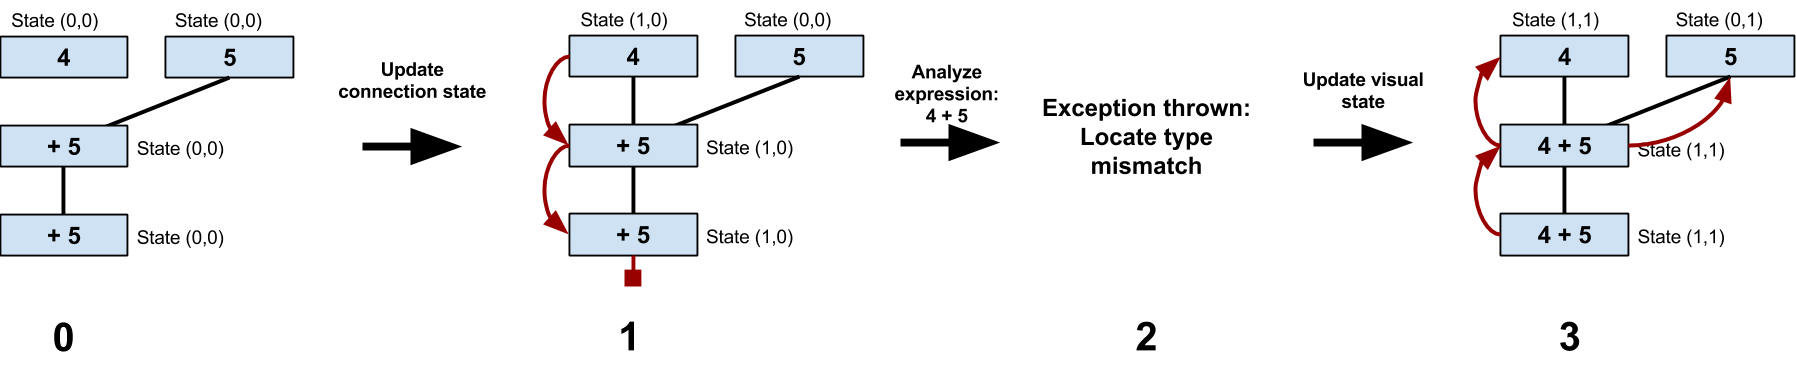
\includegraphics[width=\textwidth]{Images/invalidation}
	\caption{Invalidation scheme}
	\label{fig:invalidation}
\end{figure}

\subsection{ContextMenu}

In order to enable context specific actions in a touch environment we needed some kind of specific menu.
The CircleMenu class, an extension of the CirclePopupMenu of the JFXtras library, fulfills this role by showing a series of icons that trigger context specific actions such as copy, paste, save and delete.
As of this writing delete is the only context specific action that has been implemented.

\subsection{FunctionMenu}

The front end uses the FunctionMenu class as a main toolbar for interaction.
The menu can be called using a right click on the workspace and is constructed using a series of ListViews inside an Accordion.
Additional components have been listed inside of the Accordion as Buttons for quick and convenient access.
Each List inside of the Accordion corresponds to a catalog category in Haskell, this is done in order to make it easier for a user
to find a specific function.

\section{Back end}

\subsection{GHC integration}

The front end enables the user to construct Haskell expressions in a convenient manner.
The visual representation is converted into a tree of expression (\code{Expr}) objects and passed to the back end. \index{Expr}
The back end, finally, integrates with the Glasgow Haskell Compiler (\gls{GHC}) to do the actual computation.

The GHC integration is very simplistic.
The back end launches an instance of GHCi, the interactive read-eval-print-loop. \index{REPL}
This \gls{REPL} is then drip-fed the expressions over its standard input stream, converted from the intermediate representation into actual Haskell program code.
If the expression compiles and executes without problems, the result is returned to the front end.

\subsection{Expression and type representation}

\begin{figure}[h]
	\centering
	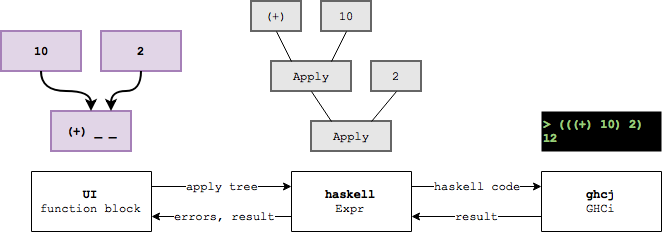
\includegraphics[scale=0.5]{Images/exprtohaskell}
	\caption{Translation from visual representation to Haskell code}
	\label{fig:exprtohaskell}
\end{figure}

\subsubsection{Expressions}
\index{function} \index{Haskell code}

To be able to work with Haskell code in Java, we built our own representation for the Haskell programming language.
We have chosen to use distinct classes (with a common superclass) for expressions that behave in a similar manner.
This object-based approach is favoured over any text based approach (including using Haskell code itself) because objects are very easy to work with.

Every expression is represented as an instance of \code{Expr} (or any subclass of \code{Expr}). \index{Expr}
An \code{Expr} is responsible for outputting syntactically correct Haskell code. \code{Expr} objects are the bridge between the tree-like graphical representation of the user interface and the textual Haskell code.
The implemented types of expressions are standard functions, values and function applications.
Each of these types of expressions share the fact that they all have a type which can be used by the type checker.

Standard functions (functions that are known to the Haskell environment) are represented as an \code{Ident} instance. \index{Ident}
This class is very simple and does not include more than the name of the function (so it can be called) and a way to lookup the type.

Values are represented in a similar way, a \code{Value} object keeps track of the string representation of the value and its type. \index{Value}
The string representation of the value should be written in a way that GHCi natively understands what is meant by it, although this is not validated.

Function application is done by using an \code{Apply} object. \index{Apply}
This class holds two expressions where the second expression is applied to the first expression.
\code{Apply} is limited to the application for a single argument.
A function with more than one argument is seen as a function with one argument that produces another function.
This way \code{Apply} allows for creating a tree like structure of a Haskell program.

Custom functions can be built using a composition of standard functions.
A custom function is defined using a \code{Function} object.
This object requires a specification of the function arguments and the expression tree of the function.
A \code{FunctionArgument} object can be used in this expression tree to use the inputs.
Functions that are defined this way will make sure that type calculations are done on a per-usage basis so reusing a function is always possible.
When a function is pushed to GHCi an \code{Ident} object is given which can be used instead of the \code{Function} object.
This comes with a great performance gain because the function itself is not continuously type checked.

Once a program has been represented as a tree of \code{Expr} objects, calling the \code{Expr.analyze()} method will invoke the type checker.
The type checker calculates the new types for the expressions in the tree.
The new types of each expression can be obtained by calling the \code{Expr.getType()} method.
This way it is possible to always get the up-to-date type of an \code{Expr} object by simply keeping a reference to it.

\begin{figure}[h]
\centering
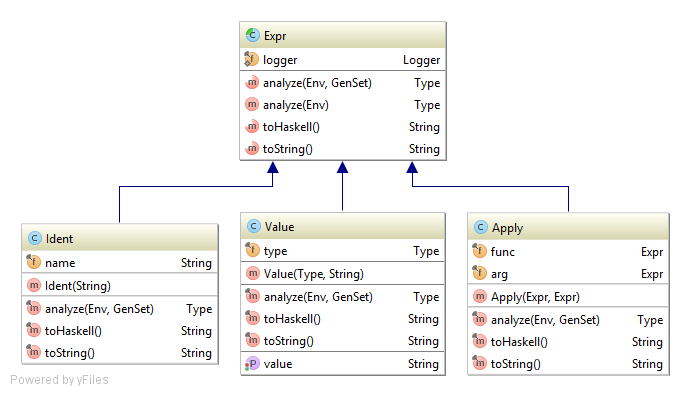
\includegraphics[scale=0.4]{Images/classdiagram-expr}
\caption{Class diagram of the Haskell expressions classes}
\label{fig:classdiagram-expr}
\end{figure}

\subsubsection{Types}
\index{type}

Types are represented similarly to expressions.
Each type is represented as an instance of \code{Type} (or any subclass of it).
The subclasses of \code{Type} are used to make working with types easier.
There is no subclass for every distinct type in Haskell, only for groups of types that are alike.

First of all types are separated into two groups: variable types and non-variable types.
Variable types are types of which the actual type is not known - types that can unify into any non-variable type (possibly with constraints).
Variable types are represented as \code{VarT}.

Non-variable types (constant types) are represented as \code{ConstT} and consist of a type constructor and a number of (optional) argument types.
A type is considered constant when it is clear which type constructor to use. A type with a known type constructor but variable types as argument types is still a constant type.

Composite types, e.g. list and tuple, are represented by respectively \code{ListT} and \code{TupleT} which are subclasses of \code{ConstT}.
These subclasses handle some validation and Haskell/string representation that is specific to these types.

Distinct Haskell types are represented as class instances, not as the class itself. The different \code{Type} subclasses make it easier to work with the types, and some are necessary in case of compound types like \code{ListT} and \code{TupleT} which are special cases.

Non-variable types can be easily compared. Two instances of the same type are equal (that is, two instances with the same base class and constructor arguments).
Variable types are only equal if it is the same instance. This is used to avoid confusion between variable types with the same name.

Type classes are represented as \code{TypeClass} instances and can be used as constraints on variable types.
Each \code{TypeClass} instance keeps a set of constant types that belong to the type class.
This information is used by the type checker to check whether a variable type is unifiable with a constant type or another variable type.

\begin{figure}[h]
\centering
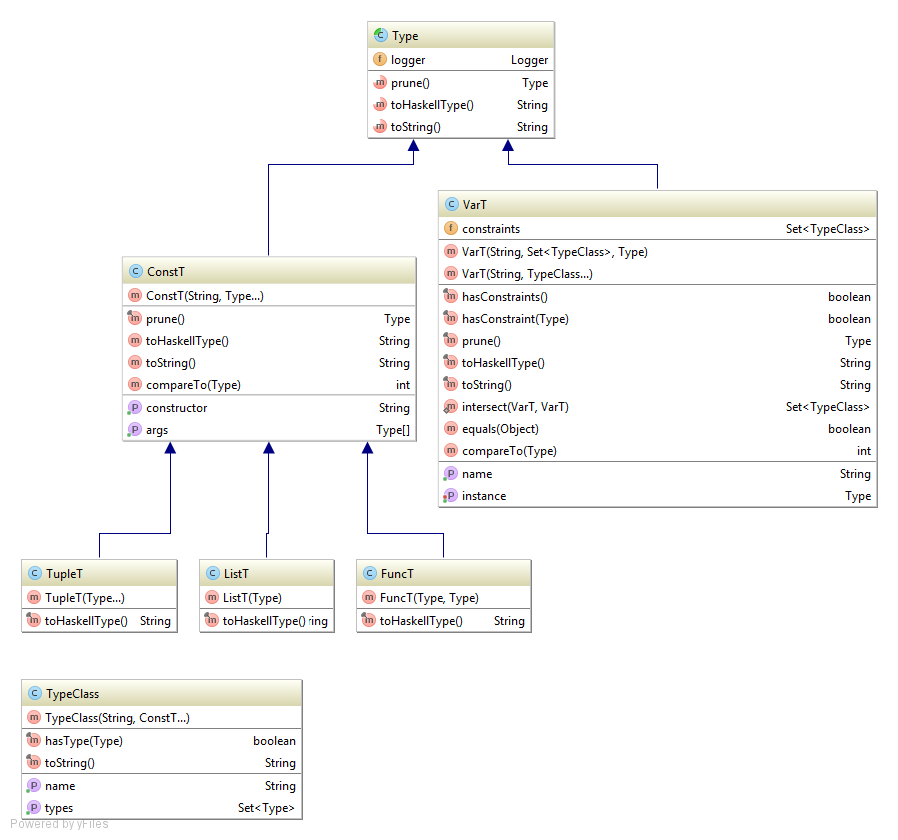
\includegraphics[scale=0.4]{Images/classdiagram-type}
\caption{Class diagram of the Haskell types classes}
\label{fig:classdiagram-type}
\end{figure}

\subsection{Type checker}
\index{type checker}

From our own experience as beginning Haskell programmers, we often encountered type errors, and therefore GHC's type error messages.
Very early in the project, we decided that the back end had to do at least some type-related work itself, to provide better errors to the user, and also to be able to show type hints, without having to parse GHC's error messages.
Not long thereafter, it was decided that such a home-grown type checker would not need to support the entirety of Haskell's type system.

After some iterations, we have arrived at an approach that could probably be described as a subset of Hindley-Milner type inference. \index{Hindley-Milner} \index{type inference}

Our (Java) implementation of Hindley-Milner type inference is based on an implementation in Scala by Andrew Forrest\cite{forrest}.
This implementation was in turn based on an implementation in Perl by Nikita Borisov\cite{borisov}.
The Perl implementation was heavily inspired by a Modula-2 implementation from 1987 by Luca Cardelli\cite{cardelli}.
Some ideas were also taken from the chapter on types from the programming languages book by Krishnamurthi\cite{plai}.

As mentioned, the type checker is not nearly powerful enough to understand or even represent the entire complexity of Haskell's type system.
However, we have found it to be `good enough' for our purposes.

\subsection{Environment management}
\index{catalog}
\index{environment}

In Haskell a lot of things depend on the environment, for example the functions that are available, the types in type classes, etc.
Our implementation solves this by introducing an environment (\code{Env}).
Objects of this class keep the types of the available functions and the type classes for every type.
Furthermore, we provide a XML-based catalog where the initial functions and type classes can be configured.
This catalog contains information that can be used by the front end, such as documentation as well.


\chapter{Test Plan}
\index{test plan}

To test the finished product, we used (automatic) unit tests as well as (manual) acceptance tests.
The unit tests mainly cover the back end of the application because it is difficult to unit test the front end, mainly because of the user interface.
The acceptance tests are focused on the front end.

\section{Acceptance tests} \label{acceptance tests}
	\subsection{Test 1}
		This test evaluates the functioning of the FunctionMenu and the spawning of basic blocks.
		
		\begin{enumerate}
			\item Right click on the workspace to open the FunctionMenu.
			\item Click on the item labelled Basic.
			\item Observe that contents are present in the opened list.
			\item Click on the Basic item again to close the list.
			\item Press the button at the bottom of the menu labelled Value Block.
			\item Enter "Hello" into the opened dialog window (using quotation).
			\item Confirm the presence of a block labelled "Hello" in the workspace.
		\end{enumerate}
		
	\subsection{Test 2}
		This test is a follow up to Test 1 and will evaluate the functioning of the context menu
		and the delete function.
		
		\begin{enumerate}
			\item Right click on the workspace to open the FunctionMenu.
			\item Press the button at the bottom of the menu labelled Value Block.
			\item Enter "DeleteMe" into the opened dialog window (using quotation).
			\item Confirm the presence of a block labelled "DeleteMe" in the workspace.
			\item Select the "DeleteMe" block by left clicking on it.
			\item Right click on the selected block to open the context menu.
			\item Click on the scissor icon.
			\item Confirm that the "DeleteMe" block has been removed from the workspace.
		\end{enumerate}
		
	\subsection{Test 3}
		This test will evaluate the functioning of the plus operator FunctionBlock and the Display Block.
		
		\begin{enumerate}
			\item Right click on the workspace to open the FunctionMenu.
			\item Press the button at the bottom of the menu labelled Value Block.
			\item Enter the number 5 into the opened dialog window.
			\item Confirm the presence of a block labelled 5 in the workspace.
			\item Repeat steps 2,3 and 4.
			\item Click on the item labelled "Numeric Types".
			\item Observe that contents are present in the opened list.
			\item Select the entry in the list labelled "(+)".
			\item Confirm that a FunctionBlock titled "(+)" has been made in the workspace.
			\item Left click on the bottom anchor on one of the ValueBlocks and drag a line all the way to one of the upper anchors of the (+) FunctionBlock.
			\item Repeat the previous step for the other ValueBlock.
			\item Click on the button at the bottom of the FunctionMenu labelled Display Block.
			\item Confirm that creation of a DisplayBlock in the workspace.
			\item Left click on the bottom anchor of the (+) FunctionBlock and drag a line all the way to the upper anchor of the Display Block.
			\item Confirm that the Display Block now displays the value 10.
		\end{enumerate}
		
	\subsection{Test 4}
		This test will verify that the the type evaluation of Viskell is working accordingly.
		
		\begin{enumerate}
			\item Right click on the workspace to open the FunctionMenu.
			\item Press the button at the bottom of the menu labelled Value Block.
			\item Enter the value False into the opened dialog window.
			\item Click on the item labelled "Numeric Types".
			\item Observe that contents are present in the opened list.
			\item Select the entry in the list labelled "(+)".
			\item Confirm that a FunctionBlock titled "(+)" has been made in the workspace.
			\item Connect the output of the Value Block with the FunctionBlock.
			\item Confirm that the argument in the FunctionBlock and the Connection line are highlighted red.
		\end{enumerate}
	
	\subsection{Test 5}
		This test will evaluate the functionality of higher order functions, knots and GraphBlocks as defined in Viskell.
		
		\begin{enumerate}
			\item Right click on the workspace to open the FunctionMenu.
			\item Press the button at the bottom of the menu labelled Graph Block.
			\item Select the entry in the FunctionMenu labelled ?Numeric Types?.
			\item	Scroll down in the newly opened list until you find the Sin function.
			\item Click on the item to create a new Sin FunctionBlock.
			\item Press the black circular knot and drag it to the left.
			\item If done correctly the FunctionBlock should now display: ((Floating a) -> (Floating a))
			\item Click on the output anchor at the bottom of the Sin FunctionBlock and drag a line to the Input anchor of the Graph Block.
			\item The Graph Block should now display the Sin function in a graphical way.
		\end{enumerate}

	\subsection{Test 6}
		This test will test the workings of the DefinitionBlock feature of Viskell, it will also illustrate the updating capacity of the GraphBlock through function translation.

		\begin{enumerate}
			\item Right click on the workspace to open the FunctionMenu.
			\item Select the entry in the FunctionMenu labelled ?Numeric Types?.
			\item Select the (*) function to create a new FunctionBlock.
			\item	Scroll down in the newly opened list until you find the Sin function.
			\item Click on the item to create a new Sin FunctionBlock.
			\item Press the button at the bottom of the menu labelled Graph Block.
			\item Press the button at the bottom of the menu labelled Slider Block.
			\item Press the button at the bottom of the menu labelled Definition Block.
			\item In the opened dialog window input: ?trans :: Float -> Float? and press enter.
			\item Left click on the upper input anchor of the Definition Block and drag a line to the left input anchor of the (*) function.
			\item Left click on the output anchor of the Slider Block and drag a line to the right input anchor of the (*) function.
			\item Left click on the output anchor of the (*) function and drag a line to the input anchor of the Sin function.
			\item Left click on the output anchor of the Sin function and connect it to the bottom input anchor of the Definition Block.
			\item Left click the output anchor of the Definition Block and connect it to the input anchor of the Graph Block.
			\item Confirm that the connections between all the blocks are working by observing a red line along the X-axis of the Graph Block.
			\item Drag the slider of the Slider Block slowly to the right and observe the output in the Graph Block.
			\item If done correctly you should have observed the increase in frequency of the Sin function.
		\end{enumerate}

\section{Unit tests} \label{unit tests}

A large part of the back end is covered by unit tests.
Almost all tests focus on the Haskell representation to make sure that the Haskell code generated by the program is as expected.
The type parser is also tested extensively to make sure types are consistent and no invalid type errors are raised.

The following parts are covered by the unit tests:

\begin{enumerate}
	\item GHCJ
	\begin{enumerate}
		\item Evaluating expressions
		\item Retrieving expressions
	\end{enumerate}
	\item Haskell catalog
	\begin{enumerate}
		\item Parsing of categories
		\item Parsing of default functions
		\item Parsing of type classes
	\end{enumerate}
	\item Expressions
	\begin{enumerate}
		\item Haskell code representation
		\item Types of expressions
		\item Inferred types of expressions
	\end{enumerate}
	\item Types and type classes
	\begin{enumerate}
		\item Haskell signature representation
		\item Type propagation
		\item Type inference: unification
		\item Type inference: pruning
		\item Deep copying
		\item Equality
	\end{enumerate}
	\item Type parser
	\begin{enumerate}
		\item Parsing of constant types, variable types with and without type classes, function types, list types, tuple types
		\item Parsing of complex, combined types
	\end{enumerate}
\end{enumerate}

The tests are not described in detail here, the exact test cases are included in the source code.


\chapter{Evaluation}
\label{chap:Evaluation}

\section{Product}

% Did we build what we wanted to build?
% Maybe include user tests here? Let our moms program Haskell for a bit?

\section{Process}

On the technical tools side, none of the members on the team had extensive experience with git \emph{and} GitHub \emph{and} Maven \emph{and} Travis, and some had never used either. It took quite a while for some to `get' the proposed workflow, and there was a lot of friction, many hours lost, and some frustration with those who struggled. Presentations on the subject helped, but some friction remained.

On a few occasions, we had difficulties planning sprints. Sprint goals and requirements either turned out to be vague at the end of the sprint, making it unclear or disputed whether or not we had completed them, or the goals were missed altogether.




\chapter{Conclusions}



\chapter{Recommendations}
\index{recommendations}

Wile working on this project we came up with a lot of ideas.
Sadly, a large number of these ideas were too big or too complicated to be included in this project.
However, future developers might find these ideas useful as inspiration.

We have compiled a wish list of the features we would like to see in Viskell:

\begin{itemize}
	\item Circular menu (see \ref{circular_menu} on page \ref{circular_menu}).
	\item Compact view of functions (for large programs).
	\item Full multi-touch controls for everything.
	\item Advanced user interface functions such as snapping and a mini-map.
	\item Search functions in menu.
	\item Support for more Haskell functions (e.g. I/O).
	\item Support for explicit recursion and pattern matching.
	\item Support for custom data types.
	\item Better support for multiple errors.
	\item The ability to input Haskell code and/or loading Haskell code.
	\item Undo and redo.
	\item Save and load programs.
	\item Larger canvas (currently not possible due to an issue with OS X).
	\item Preferences menu for some user interface behaviour.
\end{itemize}


\printindex

\printglossaries

\bibliographystyle{unsrt}
\bibliography{Chapters/Bibliography}

\begin{appendices}
\chapter{User Guide}
\label{chap:Guide}

\section{Developer guide}

This part of the document provides some information to developers on how to use and extend the functionality of the program.

\subsection{Haskell back-end}

\subsubsection{Types}

All types are an instance of a subclass of the \code{Type} class. Haskell types \emph{should} where possible be implemented as a class instance instead of a class itself.
This will mostly be \code{ConstT} as this class can be used for almost anything with a type constructor.

Non-variable types can be easily compared. Two instances of the same type are equal (that is, two instances with the same base class and constructor arguments).
Variable types are only equal if it is the same instance. This is used to avoid confusion between variable types with the same name.

\subsubsection{Expressions}

All kinds of expressions inherit from the \code{Expr} class.

\subsubsection{Catalog}

Extending the catalog should be straightforward.
An XSD (XML Schema Definition) is provided for the catalog XML file describing the layout of the file. Catalog files can be validated against this XSD.

Make sure that the software is capable of handling a type, typeclass or function before (permanently) adding it to the catalog.

\subsection{User interface}

\end{appendices}

\end{document}
